\documentclass{article}
\usepackage[utf8]{inputenc}
\usepackage[T1]{fontenc}
\usepackage{microtype}
\usepackage{graphicx}
\usepackage{booktabs}
\usepackage{amsmath,amssymb}
\usepackage{hyperref}
\newcommand{\theHalgorithm}{\arabic{algorithm}}
\usepackage{icml2026}
% Working-paper notice only: retain official margins/fonts and anonymous layout,
% but do not falsely state that this document is under conference review.
\makeatletter
\renewcommand{\Notice@String}{Working draft, November 2026. ICML-style evidence
checkpoint; not submitted or accepted.}
\makeatother
\usepackage{array}
\usepackage{xurl}
\hypersetup{pdfauthor={},pdftitle={Action Fidelity Without Physical Qualification},
  pdfsubject={Working empirical audit manuscript; not a submitted or accepted paper},
  pdfkeywords={world models, physical grounding, action fidelity, replication}}
\newcommand{\DINO}{DINO (Point)}
\newcommand{\MSE}{\operatorname{MSE}}
\newcommand{\E}{\mathbb{E}}
\icmltitlerunning{Action Fidelity Without Physical Qualification}

\begin{document}
\twocolumn[
\icmltitle{Action Fidelity Without Physical Qualification:\\
A Replicated Diagnostic Audit of Frozen PushT World Models}
\begin{icmlauthorlist}
\icmlauthor{Anonymous Authors}{anon}
\end{icmlauthorlist}
\icmlaffiliation{anon}{Anonymous affiliation}
\icmlcorrespondingauthor{Anonymous Author}{anonymous@example.invalid}
\icmlkeywords{world models, physical grounding, diagnostic evaluation, replication}
\vskip 0.3in
]
\printAffiliationsAndNotice{}

\begin{abstract}
Action-conditioned latent predictions are often evaluated as evidence for
physical understanding and planning, but these interpretations require different
measurement and decision controls. We audit two frozen RGB PushT releases using
paired simulator trajectories, actual-image probes, persistence and action
controls, native-goal ranking, and recorded pretraining-distribution sequences.
Bounded ridge and nonlinear probes do not achieve the physical resolution needed
to interpret the original latent-editing experiment, while oracle-history
prediction does not clearly outperform aligned local persistence for the audited
DINO release on generated trajectories. A prospectively specified replication
on 128 fresh roots supports latent action-effect fidelity and specificity for
both checkpoints: four contrasts have negative 99\% intervals in a fixed
five-member primary family, whereas a discovery-stage DINO ranking advantage is
inconclusive. An eight-root numerical audit finds that encoding-layout
disagreement is strongly reduced by a convolution-precision control, without
establishing the cause of all historical numerical drift. These results provide
a checkpoint-specific empirical case study in which replicated action fidelity
coexists with unqualified physical interpretation and limited decision
evidence, rather than a new general theory or demonstrated closed-loop gain.
\end{abstract}

\section{Introduction}
\label{sec:intro}

Latent world models support planning without reconstructing every pixel, but the
meaning of a successful prediction depends on the evaluation. A representation
may distinguish actions without recovering small physical changes; a forecast
may have low latent error without selecting a useful control. Joint-embedding
models and planning systems motivate these questions
\citep{maes2026lewm,zhou2025dinowm}, while prior work already distinguishes
physical grounding, intervention validity and decision alignment
\citep{vakalis2026interventiongap,subramanian2026counterfactual,liu2026djepa}.
We apply those distinctions to an empirical audit rather than introduce them as
a new framework.

Our starting experiment asked whether physical latent edits transfer across
appearance changes. That claim requires a reliable measuring instrument and an
editor whose effects can be interpreted on the evaluated feature surface.
Neither prerequisite was established. We therefore retain the unsuccessful
qualification rather than reinterpret latent prediction accuracy as proof that
the edited states are physically correct. This motivates three concrete
questions: can bounded actual-image probes resolve physical state and paired
changes; do predictions match executed action consequences beyond simple
controls; and does the unchanged goal metric select useful candidates?

The audit evaluates the released LeWM projected-token model and an RGB
DINO-WM release supplied by the Point-LeWM authors. The latter uses dummy
proprioceptive input and is not a claim about every DINO-WM implementation.
We first run discovery diagnostics on 128 simulator roots and 128 recorded
episode windows. Follow-ups use the inspected simulator sample and are explicitly
exploratory. We then specify a fixed five-contrast family and generate 128 fresh
roots without changing the task distribution or selecting favorable seeds.

The independent sample supports action-effect fidelity and matched-action
specificity for both checkpoints, but not the DINO forecast-over-endpoint ranking
claim under its prescribed interval. Approximately half of the fresh
root--branch candidate banks have no positive goal coverage, limiting decision
interpretation. A separate, bounded numerical audit distinguishes encoding
layout, rollout layout, recurrence-wrapper and metric-reduction changes.

\paragraph{Contributions and boundary.}
We provide (i) a preserved qualification failure with actual-image, probe-capacity
and observability controls; (ii) a fixed fresh-root replication of four
checkpoint-specific latent action contrasts, together with an inconclusive
ranking result; and (iii) a controlled numerical audit and authenticated
operational record. We do not establish absence of physical information,
successful physical editing, a causal mechanism for ranking behavior, or
closed-loop improvement. The novelty sought is this bounded empirical evidence,
not priority for its component evaluation ideas.

\section{Related Work}
\label{sec:related}

\paragraph{Predictive representations and physical grounding.}
LeWM learns joint-embedding dynamics from pixels, whereas DINO-WM predicts
pretrained visual features \citep{maes2026lewm,zhou2025dinowm,oquab2023dinov2}.
The Point-LeWM study compares observation interfaces and supplies the specific
RGB release audited here \citep{oberweger2026pointlewm}. Physics probing and
physical-state grounding are established directions
\citep{joseph2026interpretingphysics,yan2026psgjepa}. A probe's failure can
reflect its capacity, observation ambiguity or distribution mismatch, not
information absence. Intervention Gap and counterfactual action evaluation
explicitly qualify measurement and observation bottlenecks before physical
interpretation \citep{vakalis2026interventiongap,subramanian2026counterfactual}.
Our negative probe findings adopt, rather than originate, that logic.

\paragraph{Internal interventions.}
Causal abstractions and temporal intervention supervision provide foundational
tests of correspondences between neural and high-level variables
\citep{geiger2021causalabstractions,lippe2022citris}. Recent world-model studies
use native counterfactual references, low-rank carriers and persistent internal
corrections \citep{liu2026latentcarriers,yao2026rolloutfaith}; geometric editable
representations address appearance-consistent semantics
\citep{huang2026geocosavi}. Divergent neural interventions can invalidate simple
probe interpretations \citep{grant2025divergent}. We report an unqualified
initial editor study, not an editor that improves upon these methods.

\paragraph{Action effects and decision quality.}
Delta-JEPA and Do-JEPA explicitly target action-sensitive representations and
interventional effects \citep{zhang2026deltajepa,resani2026dojepa}. Our
matched-action analysis is instead a diagnostic of frozen releases, with no
action-effect training. Prediction--control objective mismatch is longstanding
\citep{lambert2020objectivemismatch}; D-JEPA studies decision alignment from
predictions, realized costs and outcomes \citep{liu2026djepa}. Comparing rankings
from actual encoded endpoints and forecasts is not itself a new decision
alignment method. The broader interpretability agenda likewise distinguishes
decoding, dynamics, causal verification and action
\citep{wang2026worldmodelinterpretability}. We contribute a replicated case
study within that agenda, with unsuccessful and inconclusive outcomes retained.

\section{Experimental Design}
\label{sec:design}

\subsection{Frozen Checkpoints and Interfaces}
LeWM exposes a 192-dimensional projected CLS representation. The audited DINO
release exposes 196 DINOv2 ViT-S/14 patch tokens, each 384-dimensional, with
auxiliary channels handled by its native recurrence. We score visual features,
not a decoded RGB forecast. Images are resized to $224\times224$ and each
released normalization is applied once. DINO then natively resizes the normalized
224-pixel image to 196 pixels before its 14-pixel patch encoder, producing
$14\times14=196$ tokens; the audit RGB surface and encoder input are distinct.
Models remain frozen and in evaluation
mode; inference is float32 on an RTX PRO 6000 Blackwell GPU with PyTorch
2.10.0+cu128. Source, weight and normalization hashes are fixed (Appendix
\ref{app:artifacts}). Raw latent magnitudes across these spaces are not model
rankings.

\subsection{Paired Simulator and Recorded Data}
\label{sec:data}
PushT follows the released simulator lineage
\citep{chi2023diffusionpolicy,maes2026stableworldmodel,oberweger2026pointlewm}.
A simulator root defines a factual and counterfactual initial-condition branch,
with position or orientation intervention applied before the observation
history. Both branches execute the same eight action candidates and are
rerendered with original, color-only and background-only appearances, without
changing their physics. The 512-unit arena and angular labels provide native
physical ground truth; these units are not resized-image pixels.

Three history frames occur after primitive controls 0, 5 and 10. Each action
chunk packs five ordered XY controls; two chunks connect the history, followed
by eight future chunks. Thus horizon 8 ends after 50 primitive controls,
including the ten-control prefix. Candidate 0 is hold; the bank also contains
approach, away and fixed-seed smooth random/biased controls. Trajectories are
not shortened upon native success. Apart from the original initial-geometry
rejection rule, no outcome-based rejection or replacement is allowed.

The original sample has 256 editor, 128 scorer, 64 validation and 128 pilot roots.
Actual-image probes fit scorer roots and select only on validation roots. All
seeds and pilot candidates are retained. The recorded diagnostics use 128
authenticated episode/start windows from the released PushT expert-training
dataset, identical for both models. Finite terminal action labels and finite
nonterminal controls outside the native unit box are preserved without clipping;
terminal rows never become outgoing transitions. This is a
\emph{pretraining-distribution diagnostic}, not held-out generalization.

\subsection{Discovery, Replication and Experimental Unit}
\label{sec:uncertainty}
Discovery diagnostics and follow-ups use the same 128 inspected pilot roots.
Their 5,000-draw intervals are pointwise 95\% root/episode bootstrap intervals,
not simultaneous confirmation. The follow-up protocol was fixed after earlier
results but before its execution. It is not retrospective preregistration.

The subsequent replication fixes pilot seed 2026110201 and root indices 0--127
before generation. Identities are disjoint from every original split, the
originally reserved 3,384-root roster and a software-preflight root. Original
scorer/validation files are copied byte-identically but are not fitted or
encoded in this dynamics-only pass. The unchanged generator produces exactly
128 fresh roots. Both models evaluate every branch, candidate, appearance and
future step, yielding 6,144 bank/horizon records per model.

The primary slice is original appearance, horizon 8. Each bank first averages
its candidate contrasts, then the two branches are averaged within a root,
and roots receive equal weight. Candidates, branches, frames and appearances
are not independent experimental units. The five primary contrasts share
10,000 PCG64 bootstrap draws with seed 20261102. Two-sided percentile 99\%
intervals apply Bonferroni correction to a nominal 0.05 familywise level;
bootstrap coverage is asymptotic, not a finite-sample guarantee. A prescribed
negative direction is supported only if the whole interval is below zero.
All other slices and metrics remain pointwise exploratory 95\% results.

\section{Diagnostic Estimands and Controls}
\label{sec:estimands}

\subsection{Physical Measurement}
\label{sec:measurementmethods}
Actual-image probes predict pusher XY, block XY and sine/cosine angle labels.
Ridge candidates use fixed spatial pooling and regularization grids; a 64-unit
SiLU MLP uses seeds 11, 29 and 47, two weight decays and checkpoints at 50,
100 and 200 epochs. MLP feature normalization and target means are estimated
only from scorer data; target scales are fixed, not estimated. Target-group
selections use validation losses with separate fixed reporting scales (Appendix
\ref{app:probes}). Choices and weights are
published before pilot evaluation. All MLP seeds are reported, not a best seed.
The follow-up includes all candidates, unlike the earlier selected-candidate
mixed-time readout summary (Appendix \ref{app:probes}).

State distances and circular angular errors are paired with effect-error
controls. A training-mean readout implies zero change between factual and
counterfactual branches. The 4-unit/2.5-degree follow-up resolution targets are
diagnostic commitments motivated after discovery, not externally established
task tolerances. We do not reinterpret a relative improvement over a weak
baseline as adequate absolute resolution.

\subsection{Prediction and Feedback}
Let $A_{rbk,h}$ be an actual encoded future for root $r$, branch $b$, candidate
$k$, horizon $h$, and $P_{rbk,h}$ its autonomous forecast. Within a model, use
$d(x,y)=D^{-1}\lVert x-y\rVert^2$ over every audited visual coordinate.
Autonomous prediction is compared with persistence of the final initial-history
feature, and with a native zero-future-action rollout preserving the prefix.

Oracle-history predictions receive actual aligned observations at each step.
Their control is \emph{local persistence}, the immediately preceding actual
feature, not persistence of the initial frame. Otherwise oracle improvement
would conflate useful local dynamics with a much easier prediction problem.
DINO crosses free/actual visual history with recurrent/encoded-zero auxiliary
history. Reset means the native encoder applied to zero proprioception, not
literal zero channels; recurrent patch-varying outputs are retained. Oracle
observations are privileged and not a deployable forecasting improvement.

\subsection{Action-Effect Fidelity and Specificity}
\label{sec:action}
For $k>0$, define hold-relative effects
$\Delta P_k=P_k-P_0$ and $\Delta A_k=A_k-A_0$ within a bank. The fidelity contrast is
\begin{equation}
 F_{rb}=\frac{1}{K-1}\sum_{k=1}^{K-1}
 \left[d(\Delta P_k,\Delta A_k)-d(0,\Delta A_k)\right].
 \label{eq:fidelity}
\end{equation}
Negative favors the forecast over predicting no effect. Zero-effect cases
remain without denominator floors or exclusions. Specificity compares each
prediction with its corresponding actual endpoint and \emph{every} wrong
assignment:
\begin{equation}
 S_{rb}=\frac{1}{K}\sum_{k=0}^{K-1}
 \left[d(P_k,A_k)-\frac{1}{K-1}\sum_{j\ne k}d(P_k,A_j)\right].
 \label{eq:specificity}
\end{equation}
The complete $K\times K$ assignment matrix is retained; a selected shuffle is
not the control. Aggregate signed effect gain is the ratio of equal-root mean
dot product to mean true-effect energy, not the mean of unstable rootwise
ratios. Undefined bootstrap denominators are reported. These metrics establish
latent correspondence, not block-specific physical correctness.

\subsection{Finite-Bank Decisions}
\label{sec:ranking}
For each bank, apply the checkpoint's unchanged native goal score to either
actual encoded endpoints or forecasts. LeWM uses summed squared feature error
and DINO uses mean squared feature error; multiplying a within-model score by a
positive constant does not change its ranking. Ties select the smallest index.
Evaluate the chosen candidate using the saved native coverage cost
$c_k\in[0,1]$:
\begin{equation}
 R(q)=c_{\arg\min_k q_k}-\min_k c_k.
 \label{eq:regret}
\end{equation}
Hold regret is $c_0-\min_k c_k$ and expected uniform regret is
$K^{-1}\sum_k c_k-\min_k c_k$. We retain absolute best coverage and the rate
at which every candidate has zero coverage. Zero regret on such a bank is
uninformative about success. Forecast-minus-endpoint regret is primary only for
DINO; both action contrasts are primary for each model. No closed-loop task
success is asserted.

\section{Results}
\label{sec:results}

\subsection{The Physical-Editor Interpretation Remains Unqualified}
\label{sec:measurement}
The original editor pilot used a scorer fitted on mixed actual/predicted
surfaces. Original-appearance losses were 71.6784 for LeWM and 520.6246 for
DINO, against a draft scaled-loss tolerance of 0.05. Selected MLP-minus-identity
effect losses were positive (+1.0984/+7.7819) with intervals above zero.
Transport interaction intervals crossed zero. These scores under
\emph{unqualified measurement} neither demonstrate physically harmful edits nor
establish appearance-invariant editing. They are not directly comparable with
the later actual-image-only probe experiment.

\begin{table}[t]
\caption{Discovery actual-image follow-up, original appearance/horizon 8.
Block errors are native distance units; angles are degrees. All MLP seeds are
retained. Paired angular-effect error is worse than zero change for every fitted
method. Probe failures do not prove absence of physical information.}
\label{tab:probes}
\centering
\small
% Generated from authenticated reports; do not edit.
\begin{tabular}{llrrr}
\toprule
Model & Probe & Block & Angle & Effect angle \\
\midrule
LeWM & Ridge & 29.32 & 20.05 & 14.69 \\
LeWM & MLP 11 & 40.67 & 18.92 & 13.98 \\
LeWM & MLP 29 & 39.64 & 18.74 & 14.02 \\
LeWM & MLP 47 & 38.57 & 19.22 & 14.60 \\
DINO (Point) & Ridge & 32.16 & 34.83 & 22.65 \\
DINO (Point) & MLP 11 & 56.90 & 38.61 & 24.99 \\
DINO (Point) & MLP 29 & 60.29 & 37.37 & 24.90 \\
DINO (Point) & MLP 47 & 55.27 & 37.82 & 23.77 \\
\midrule
Zero-change & -- & -- & -- & 11.73 \\
\bottomrule
\end{tabular}

\end{table}

The bounded actual-image follow-up does not rescue physical resolution
(Table \ref{tab:probes}). Ridge block errors are approximately 29--32 units;
all six MLP-minus-ridge block-error intervals are positive. Every fitted
method has greater paired angular-effect error than zero angular change.
Relative improvements in other quantities therefore do not qualify small
physical edits. The result is bounded to this probe family and data surface,
not an impossibility theorem.

Observation limitations are substantive: 280 exact resized-RGB hash groups have
different state labels, covering 630 of 6,912 original-appearance samples.
The empirical single-image scaled-MSE lower bound is 3.6240. This is a bound
for the finite labeled observation sample and that scaled loss, not a population,
angular-distance or full-history bound. At horizon 8, 650/2,048 pusher circles
are wholly outside the canvas. Fully-in-canvas ridge pusher errors still average
87.20/70.93 units (LeWM/DINO). No samples are removed from primary results.

\subsection{Oracle Feedback Requires an Aligned Baseline}
\label{sec:feedbackresults}
In discovery generated trajectories, replacing autonomous feedback with actual
history reduces MSE from 0.3364 to 0.0279 for LeWM and from 0.7900 to 0.1555
for DINO. Those large reductions alone do not establish useful local prediction.
Table \ref{tab:feedback} compares oracle forecasts with local persistence.
LeWM has a negative contrast; DINO's generated contrast remains inconclusive
in both discovery and the fresh sample. The fresh-sample view is exploratory,
not an additional primary-family claim.

\begin{table}[t]
\caption{Actual-history prediction minus aligned local persistence at horizon
8. Negative favors prediction; intervals are pointwise exploratory 95\%.
Recorded sequences overlap the pretraining distribution.}
\label{tab:feedback}
\centering\small
% Generated from authenticated reports; do not edit.
\begin{tabular}{lll}
\toprule
Sample & Model & MSE contrast [95\% CI] \\
\midrule
Discovery & LeWM & -0.0094 [-0.0135, -0.0057] \\
Discovery & DINO (Point) & -0.0028 [-0.0131, 0.0072] \\
Recorded & LeWM & -0.2006 [-0.2392, -0.1649] \\
Recorded & DINO (Point) & -0.2185 [-0.2428, -0.1954] \\
Fresh roots & LeWM & -0.0112 [-0.0148, -0.0078] \\
Fresh roots & DINO (Point) & 0.0029 [-0.0070, 0.0130] \\
\bottomrule
\end{tabular}

\end{table}

Both models have clear local advantages on recorded training-distribution
windows, but this does not establish generated-task or unseen-distribution
generalization. DINO auxiliary reset changes are tiny (discovery autonomous
reset-minus-recurrent MSE about $2.05\times10^{-5}$), and do not rescue its
generated local-persistence contrast. We preserve the full visual/auxiliary
control rather than attribute the gap solely to autoregressive error.

\subsection{Latent Action Fidelity Replicates}
\label{sec:replication}
Discovery effect-error-minus-zero intervals were negative for both models,
as were matched-minus-all-wrong assignment intervals. The fresh-root experiment
supports all four action contrasts with the prespecified 99\% intervals
(Table \ref{tab:primary}; Figure \ref{fig:primary}). Neither model is trained,
selected or refitted on the fresh roots.

\begin{table*}[t]
\caption{All five primary fresh-root contrasts, original appearance/horizon 8.
Equal-root estimates and two-sided 99\% bootstrap intervals form the fixed
five-member family. Negative directions support the corresponding contrast.
The DINO ranking result is inconclusive, not a successful replication.}
\label{tab:primary}
\centering
% Generated from authenticated reports; do not edit.
\begin{tabular}{llll}
\toprule
Model & Contrast & Estimate [99\% CI] & Prespecified decision \\
\midrule
LeWM & Effect vs. zero & -0.3753 [-0.4529, -0.3035] & Supported \\
LeWM & Matched vs. wrong & -0.5180 [-0.5842, -0.4544] & Supported \\
DINO (Point) & Effect vs. zero & -0.2364 [-0.2889, -0.1834] & Supported \\
DINO (Point) & Matched vs. wrong & -0.5605 [-0.5968, -0.5245] & Supported \\
DINO (Point) & Forecast vs. endpoint & -0.0071 [-0.0189, 0.0051] & \textbf{Inconclusive} \\
\bottomrule
\end{tabular}

\end{table*}

\begin{figure*}[t]
\centering
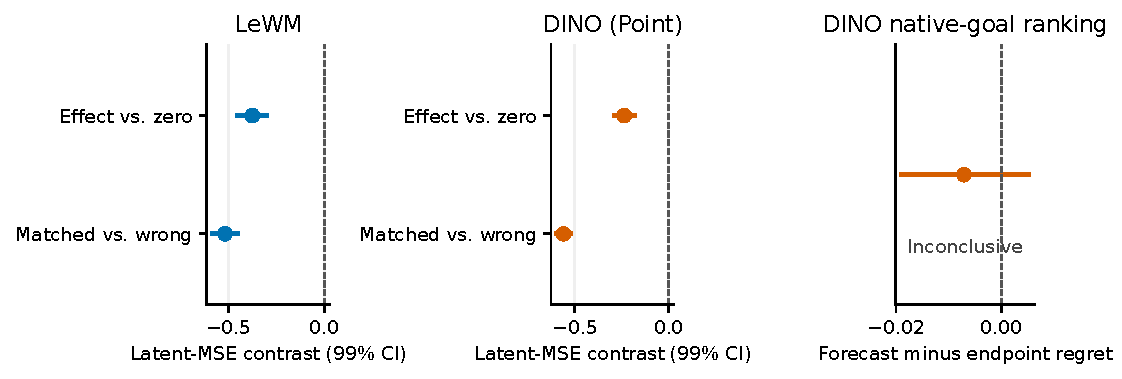
\includegraphics[width=\textwidth]{generated/replication_primary.pdf}
\caption{Fresh-root primary results. Both action contrasts are supported for
each model; DINO forecast-minus-endpoint regret spans zero. Separate latent
axes are intentional: raw magnitudes do not rank the models. All 128 roots,
both branches and all candidates contribute; no outcome-based filtering.}
\label{fig:primary}
\end{figure*}

Fresh-sample signed gains are 0.7649 for LeWM and 0.6644 for DINO, with
pointwise 95\% intervals below one and no undefined bootstrap denominators.
These ratios do not imply simply insufficient amplitude: discovery predicted/
true effect-energy ratios were approximately 1.017/1.089. Directional and
off-axis errors can coexist with similar total energy. More importantly,
neither a negative fidelity contrast nor a positive signed gain identifies
which physical component is accurately represented.

\subsection{Ranking Evidence Is Limited by Both Uncertainty and Coverage}
\label{sec:decisionresults}
The discovery DINO forecast-minus-endpoint regret was $-0.01356$ with a
pointwise 95\% interval below zero. The fresh estimate is $-0.00711$, but its
primary 99\% interval spans zero. Therefore the discovery observation is not
promoted to independently supported decision evidence. This change is not
proof that the underlying effect is exactly zero; both sample variation and
the stronger prespecified interval matter. We do not extend the sample or
search for a seed that reproduces the discovery interval.

\begin{table}[t]
\caption{Fresh-root finite-bank rankings, original appearance/horizon 8.
Regrets are native coverage-cost units. The paired forecast-minus-hold contrast
has a pointwise exploratory 95\% interval; neither interval is wholly negative.}
\label{tab:ranking}
\centering\small
\begingroup
\setlength{\tabcolsep}{3pt}
% Generated from authenticated reports; do not edit.
\begin{tabular}{lrrl}
\toprule
Model & Endpoint & Forecast & Forecast--hold [95\%] \\
\midrule
LeWM & 0.0201 & 0.0304 & 0.0034 [-0.0047, 0.0116] \\
DINO (Point) & 0.0308 & 0.0237 & -0.0033 [-0.0127, 0.0046] \\
\bottomrule
\end{tabular}

\endgroup
\end{table}

Expected uniform regret is 0.05083 and hold regret is 0.02701 on the fresh
banks. Forecast rankings show advantages relative to expected uniform choice,
but neither establishes a forecast-over-hold gain under the paired interval.
All 129/256 zero-coverage banks remain, compared with 127/256 in discovery.
Their weak candidate support limits discrimination among decision rules. A
redesigned reachable/contact-rich bank would change the estimand and needs a
new prospective study, not retrospective removal of misses.

\subsection{Execution Layout Has a Measurable Numerical Effect}
\label{sec:numerics}
The old diagnostics encoded context in batches of four then two frames and
rolled out one candidate at a time. The follow-up encoded all six context frames
together, future frames in batches of 32, and eight-candidate banks. Historical
individual native errors differed by up to 0.028922/0.013884; aggregate
native/persistence changes were at most 0.000146. We retain this discrepancy.

The numerical audit fixes the first eight original manifest entries and crosses
the observed encoding and rollout layouts, retaining actual wrapper and public
parity calls. Each model produces 7,680 comparison rows. Unchanged same-process
repeats are exact. Encoding differences dominate baseline observed-path changes;
rollout-layout effects are much smaller (Table \ref{tab:numerics}). Public and
feedback-wrapper outputs agree exactly. Metric reduction alone is zero for
LeWM and near float32 rounding scale for DINO.

\begin{table}[t]
\caption{Maximum absolute change in horizon-8 native MSE on the fixed eight-root
numerical sample. These are arithmetic/layout contrasts, not physical accuracy.
Convolution IEEE is a controlled precision permission, not a new selected model.}
\label{tab:numerics}
\centering\small
% Generated from authenticated reports; do not edit.
\begin{tabular}{lrr}
\toprule
Comparison & LeWM & DINO \\
\midrule
Observed paths & 4.90e-03 & 1.53e-03 \\
Encoding only (single) & 4.89e-03 & 1.52e-03 \\
Rollout layout (new encoding) & 2.56e-06 & 9.54e-06 \\
Wrapper vs. public & 0 & 0 \\
Metric reduction only & 0 & 1.19e-07 \\
Observed paths, conv. IEEE & 2.56e-06 & 6.44e-06 \\
\bottomrule
\end{tabular}

\end{table}

Changing convolution precision permission from TF32 to IEEE reduces maximum
observed-path MSE disagreement by about 1,910-fold/238-fold. Matmul IEEE and
cuDNN deterministic controls produce no observed change; explicit matmul TF32
does. Benchmark-off is already set and is explicitly skipped rather than
presented as an executed intervention. Parameters, all buffers including
nonpersistent masks, and restored backend properties are checked. This
establishes controlled numerical sensitivity on the bounded sample, not the
cause of every historical maximum or improved physical prediction. Both
forecast and encoded reference tensors can shift.

\section{Discussion and Limitations}
\label{sec:discussion}
\paragraph{What survives the original hypothesis.}
The physical editor-transfer claim remains unsupported because its measuring
instrument and edited feature surface were not qualified. The independent
positive findings concern latent action correspondence. Their coexistence with
poor physical readouts is an empirical observation, not a theorem that latent
fidelity precludes or guarantees physical understanding. A qualified history-
based readout could change the interpretation without invalidating the archived
negative result for the original single-image probes.

\paragraph{Scope of decision evidence.}
We neither prove a causal decomposition of ranking error nor demonstrate
closed-loop control. Actual-endpoint ranking is a privileged diagnostic, not a
deployable policy, and the limited bank may fail to offer a useful action.
The fresh DINO ranking interval is inconclusive. Broader reachable-bank or
closed-loop gains require a new design and cannot be inferred from latent
effect fidelity alone.

\paragraph{Generalization and multiplicity.}
There is one environment, two specific unmatched releases, one generated bank
distribution and a recorded pretraining-distribution sample. We cannot attribute
differences causally to architecture or rank models using their raw latent
errors. Follow-ups reuse inspected discovery data; only the fixed five fresh-root
contrasts receive primary-family inference. The 99\% bootstrap intervals offer
nominal/asymptotic multiplicity control, not guaranteed finite-sample coverage.
All other results, including fresh feedback and appearance/horizon curves, are
exploratory. The bounded probe search does not reproduce every original paper's
probing protocol.

\paragraph{Numerical and verification boundary.}
Same-process repeatability does not establish portability across devices,
caches, drivers or historical concurrent workloads. Raw latent tensors were not
archived. Independent verification recomputes every CSV summary, candidate-
level algebra, ranking choice, bootstrap interval and recorded physical/coverage
quantity from saved data; it cannot regenerate all latent measurements without
rerunning the models. Hash integrity is not a substitute for scientific validity.

\section{Conclusion}
\label{sec:conclusion}
On two frozen PushT releases, action-effect fidelity and matched-action
specificity replicate on a fixed independent sample, while physical-edit
interpretation remains unqualified and a discovery ranking advantage does not
receive independent primary-family support. A bounded backend audit further
shows that numerical layout must be controlled even with immutable checkpoints.
The resulting case study argues for reporting the precise level of evidence
earned by an experiment, including failed prerequisites and inconclusive
decisions, rather than turning predictive success into broader physical or
control claims.
\label{maintextend}

\section*{Impact Statement}
This work concerns evaluation methodology for simulated manipulation and frozen
world models. Its intended benefit is more careful separation of predictive,
physical and decision claims. Misinterpreting small latent errors or finite-bank
regret as safe physical control could encourage unreliable deployment; our
results do not justify deployment on real robots. We use released model and
simulation artifacts, not human-subject data. Redistribution of checkpoints,
datasets and upstream code remains subject to their respective terms. Scientific
and attribution checks, author approval, applicable AI-assistance disclosure and
the actual target venue's requirements are necessary before submission.

\bibliography{references}
\bibliographystyle{icml2026}
\clearpage
\appendix
\onecolumn
\section{Artifact Identity and Reproducibility}
\label{app:artifacts}

The experimental record includes exact source/configuration snapshots, fixed
rosters and input hashes, selection/plan publication before evaluation, per-stage
logs, timestamped status events, bootstrap draws and complete report/data
inventories. Output directories are exclusive: no implicit overwrite or resume
is used. Numerical failures stop execution; they do not authorize replacement
roots. Completed and failed/inconclusive scientific outcomes are different
notions. An anonymous release must be prepared before any actual submission;
this working PDF intentionally omits identifying project and sandbox links.

\begin{table}[h]
\caption{Released artifact identities. These upstream identities identify the
audited checkpoints, not an architecture-wide comparison. SHA256 values are
included in the accompanying authenticated evidence ledger.}
\centering\small
\begingroup
\setlength{\tabcolsep}{3pt}
\begin{tabular}{lll}
\toprule
Component & Upstream source/release & Pinned revision \\
\midrule
LeWM source & \texttt{lucas-maes/le-wm} & \texttt{8edfeb336732b5f3ce7b8b210d0ba370a09e2cac} \\
LeWM weights & \texttt{quentinll/lewm-pusht} & \texttt{22b330c28c27ead4bfd1888615af1340e3fe9052} \\
Point implementation/simulator & \texttt{fafraob/point-lewm} & \texttt{1b5a90ebf63e8ef165b1dfe100b81b12f4fa1424} \\
RGB DINO release & \texttt{fafraob/point-cloud-pusht} & \texttt{664278a4c0b4c5f607d0993744986b2d10b4168e} \\
DINOv2 source & \texttt{facebookresearch/dinov2} & \texttt{85a24602099d397264d5b30461ad7f3bfd726ca1} \\
Recorded PushT data & \texttt{quentinll/lewm-pusht} & \texttt{655cd446b9929369d7d406001da85c15d1457850} \\
\bottomrule
\end{tabular}
\endgroup
\end{table}

The original DINO release did not record its hub backbone source revision; the
explicit audit pin fixes that ambiguity rather than claiming it was originally
recorded. Auxiliary recurrence uses the released embedding, including its
nonzero output for zero raw proprioception. Optional xFormers is disabled;
native PyTorch attention is used. LeWM and DINO action normalization uses the
released population statistics once. Recorded actions are not silently clipped
to the native generated-control box.

Hosted inference uses Python 3.11, PyTorch 2.10.0+cu128 and a 97,887-MiB RTX PRO
6000 Blackwell Server Edition. CPU-only contract tests and report/PDF analysis
are distinct from research inference. The complete implementation suite at the
execution checkpoint contains 1,312 passing tests, no failures or skips. Tests
check invariants and real-checkpoint interfaces, not empirical success. The
tracked pending batch ran in about 23.34 minutes including numerical controls,
input authentication, generation, both model evaluations, analysis and backups.
LeWM and DINO fresh model stages took 131.57 and 570.18 seconds, respectively.
These are observed wall times, not controlled cross-model speed benchmarks.

Four pending-stage/operations ZIPs were copied off-host and strictly restored,
with 610 inventory entries verified in total. Their complete data include 128
fresh pilot and 192 copied development-root archives; repeated source snapshots
are counted as inventory entries, not independent data. Independent verifiers
recompute numerical summaries from every CSV row and replication intervals
from every complete bank. Neither loads checkpoints nor simulates new roots.

\section{Probe Selection, Observability and the Initial Failure}
\label{app:probes}

Ridge pooling grids are 4 and 7 with regularization
$\{0.01,1,100,10000\}$. LeWM's global projected token makes spatial pooling
degenerate; it is not assigned DINO's patch geometry. MLP pooling grid is 4,
hidden width 64 with SiLU, learning rate 0.001, batch size 128, weight decay
$\{0,0.01\}$ and checkpoints at epochs $\{50,100,200\}$. Seeds
$\{11,29,47\}$ use isolated initialization and shuffle streams. Selections
are target-group-specific and based on original-appearance validation roots,
with canonical ties and no pilot-based best-seed choice.

The MLP standardizes feature coordinates using scorer means and population
standard deviations, replacing deviations at most $10^{-6}$ by one. Its
targets use scorer means and fixed training scales
$s_{\mathrm{MLP}}=(512,512,512,512,1,1)$. Separately, validation/reporting and
the empirical ambiguity calculation use
$s_{\mathrm{report}}=(32,32,32,32,0.25,0.25)$ on the six XY/sine/cosine labels.
The scaled squared loss is a \emph{sum}, not an average over coordinates:
\begin{equation}
 L_s(\hat y,y)=\sum_{j=1}^{6}\left((\hat y_j-y_j)/s_j\right)^2.
\end{equation}
Target-group selection uses its group's summands, with equal-root aggregation.
Native-distance/angular metrics are reported separately. Thus the draft 0.05
scaled-loss gate and the empirical 3.6240 lower bound are not errors in degrees
or arena units, and are not the MLP training-loss scale.

Training/validation use both branches, context/future horizons and candidate
index equal to root index modulo eight. Pilot evaluation uses every candidate,
both branches and every appearance. At original appearance it contains 6,912
image samples, including 2,048 horizon-8 samples. The prior prerequisite
readout used a selected-candidate mixed-time summary of 1,536 images; the two
tables do not measure identical sample averages. The original editor pilot
also used mixed actual and predicted scoring surfaces. Its reported scaled
losses must not be compared numerically as though they were the later native
distance MAEs.

For an exact resized RGB observation $x$ with multiple scaled physical labels
$y$, the minimizing deterministic single-image squared-loss predictor is the
within-$x$ mean. Summing the within-group variance over this empirical labeled
sample gives the reported lower bound 3.6240. That statement concerns exact
pixel matches and the defined squared loss only. It is not a population
irreducible-error estimate or a lower bound for history input, angular MAE,
Euclidean distance or a differently constructed dataset. Geometric off-canvas
counts likewise do not certify semantic invisibility or justify excluding
samples after observing outcomes.

The unresolved original editor-transfer hypothesis remains in the evidence
record. Positive MLP-minus-identity scored effect loss under an unqualified
scorer does not establish physically harmful edits. Transport interaction
intervals spanning zero neither establish invariance nor an appearance-specific
failure mechanism.

\begin{figure}[h]
\centering
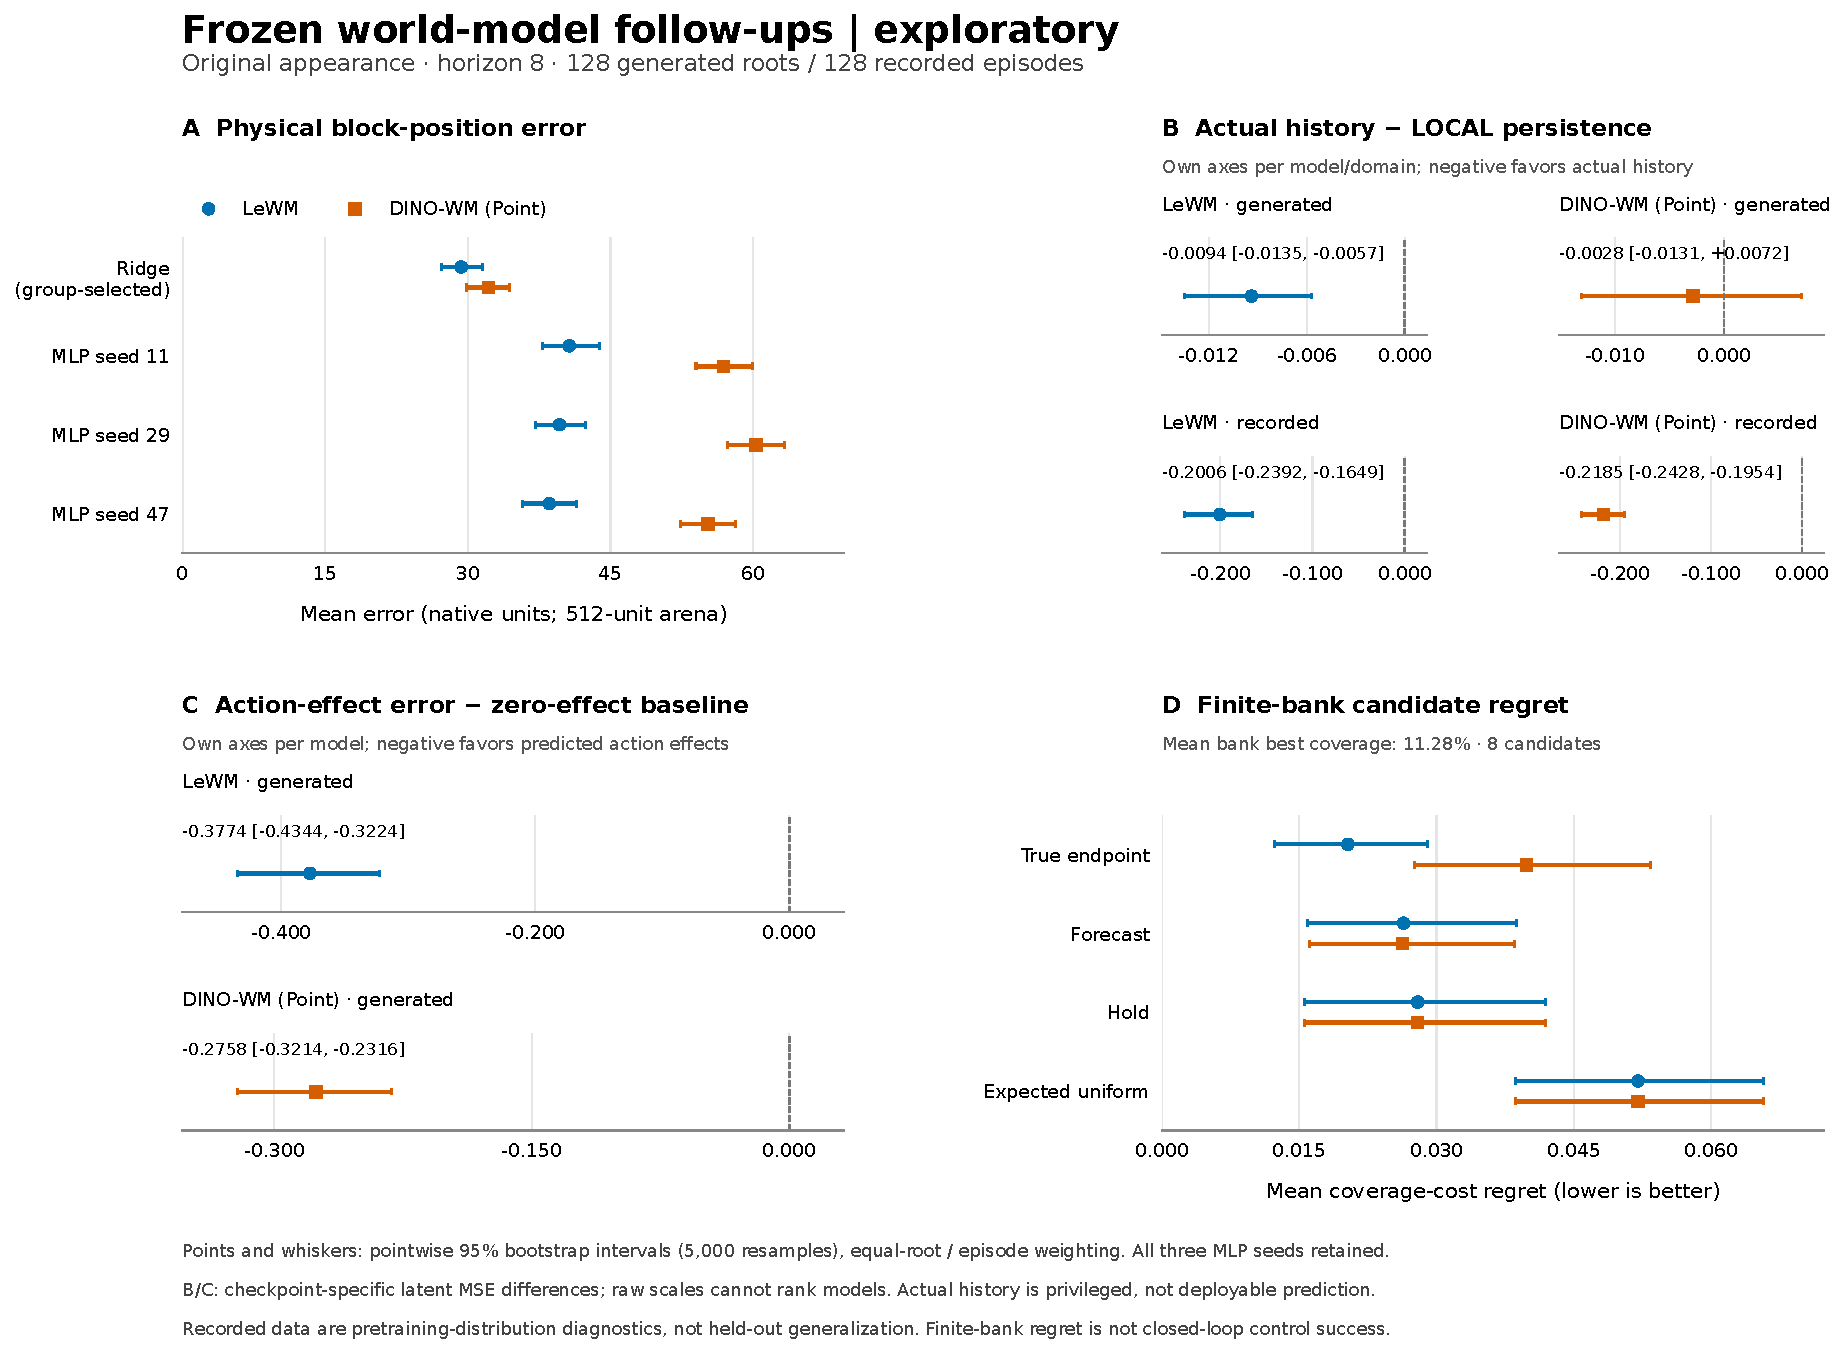
\includegraphics[width=.98\textwidth]{generated/discovery_summary.pdf}
\caption{Authenticated discovery follow-up summary. All probe seeds, oracle/
local-persistence controls, action contrasts and finite-bank regrets are
exploratory pointwise 95\% views on inspected data. These intervals must not be
read as the independent primary-family results in Figure \ref{fig:primary}.}
\label{fig:discovery}
\end{figure}

\section{Primary and Complementary Inference}
\label{app:inference}

The original manifest includes all five split names, including an empty
confirmation roster. Every original archive is authenticated before fresh-root
generation. Fresh root IDs, 128-bit root seeds and environment seeds are checked
against old and reserved identities. The generator retains the native bank,
clearance 2 and maximum 256 initial-anchor attempts; no bank improvement,
contact/visibility screening or outcome filtering is inserted.

Root means are ordered by full root ID. The saved $10000\times128$ int64
bootstrap matrix is generated once by NumPy PCG64 with seed 20261102 and used
for both models and all contrasts. Primary quantiles are 0.005/0.995, linear
interpolation. The five-member family includes Equations \ref{eq:fidelity}
and \ref{eq:specificity} for each model and forecast-minus-endpoint regret for
DINO only. Every primary estimate and interval is reported even if another
member is inconclusive. All-primary replication requires all five; that
criterion was not met.

The effect gain is $g=\overline{\langle\Delta P,\Delta A\rangle}/
\overline{\lVert\Delta A\rVert^2}$, using equal-root means after candidate
and branch averaging. If any resampled denominator is zero, the unconditional
interval is undefined and the count is reported rather than conditioning on
nonzero draws. Both fresh gains have zero undefined draws. An energy ratio
near one and $g<1$ are compatible with misaligned/off-axis effects; a
pure insufficient-amplitude explanation is not established.

The untouched underlying dynamics reports retain their legacy exploratory
schema and inspected-pilot boilerplate. Fresh sample identity and primary
inference are established by the new plan, composite data manifest and joint
analysis, not by rewriting legacy report tags. All 1,680 exploratory
estimates/intervals and five primary contrasts were independently recomputed;
maximum comparison discrepancy was $2.27\times10^{-13}$. The numerical verifier
checks 1,800 summary statistics per model with rounding discrepancy at most
$1.11\times10^{-16}$.

\begin{figure}[h]
\centering
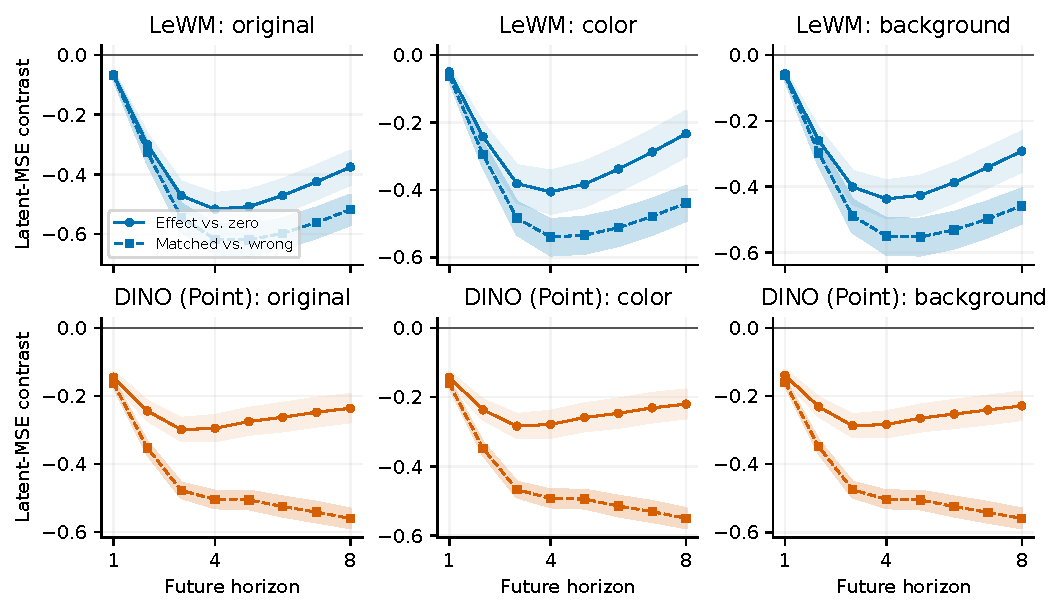
\includegraphics[width=.97\textwidth]{generated/replication_slices.pdf}
\caption{All fresh-sample horizons and appearances for the two action
contrasts. Shaded intervals are pointwise exploratory 95\%, including the
primary metrics' exploratory views. Only original appearance/horizon 8 uses
the dedicated 99\% primary family. No favorable slice is selected to replace
the inconclusive decision result. Raw latent scales remain model-specific.}
\label{fig:slices}
\end{figure}

\begin{table}[h]
\caption{Complementary fresh-sample summaries at every appearance and the
original reporting horizons. Every interval is pointwise exploratory 95\%.
Fidelity and feedback use model-specific latent MSE; forecast--hold uses native
coverage-cost regret. No row is an additional primary claim.}
\centering\small
% Generated from authenticated reports; do not edit.
\begin{tabular}{lllrrr}
\toprule
Model & Appearance & $h$ & Oracle--local persistence & Effect--zero & Forecast--hold \\
\midrule
LeWM & original & 1 & -0.0529 [-0.0633, -0.0435] & -0.0645 [-0.0762, -0.0539] & -0.0008 [-0.0038, 0.0022] \\
LeWM & original & 4 & -0.0572 [-0.0693, -0.0463] & -0.5162 [-0.5715, -0.4639] & 0.0063 [-0.0001, 0.0133] \\
LeWM & original & 8 & -0.0112 [-0.0148, -0.0078] & -0.3753 [-0.4329, -0.3221] & 0.0034 [-0.0047, 0.0116] \\
LeWM & color & 1 & -0.0389 [-0.0501, -0.0285] & -0.0493 [-0.0618, -0.0377] & -0.0010 [-0.0038, 0.0018] \\
LeWM & color & 4 & -0.0430 [-0.0559, -0.0312] & -0.4057 [-0.4695, -0.3441] & 0.0073 [-0.0012, 0.0164] \\
LeWM & color & 8 & 0.0038 [-0.0018, 0.0098] & -0.2333 [-0.2996, -0.1671] & 0.0051 [-0.0019, 0.0123] \\
LeWM & background & 1 & -0.0459 [-0.0568, -0.0363] & -0.0566 [-0.0689, -0.0457] & -0.0002 [-0.0033, 0.0028] \\
LeWM & background & 4 & -0.0532 [-0.0654, -0.0420] & -0.4374 [-0.4943, -0.3825] & 0.0076 [-0.0006, 0.0163] \\
LeWM & background & 8 & -0.0069 [-0.0109, -0.0032] & -0.2920 [-0.3531, -0.2334] & 0.0085 [0.0001, 0.0178] \\
DINO (Point) & original & 1 & -0.0625 [-0.0784, -0.0459] & -0.1450 [-0.1592, -0.1301] & -0.0016 [-0.0042, 0.0004] \\
DINO (Point) & original & 4 & -0.0015 [-0.0151, 0.0116] & -0.2953 [-0.3319, -0.2578] & -0.0079 [-0.0154, -0.0018] \\
DINO (Point) & original & 8 & 0.0029 [-0.0070, 0.0130] & -0.2364 [-0.2763, -0.1961] & -0.0033 [-0.0127, 0.0046] \\
DINO (Point) & color & 1 & -0.0575 [-0.0738, -0.0406] & -0.1425 [-0.1567, -0.1276] & -0.0007 [-0.0032, 0.0014] \\
DINO (Point) & color & 4 & 0.0049 [-0.0081, 0.0175] & -0.2787 [-0.3158, -0.2409] & -0.0080 [-0.0155, -0.0020] \\
DINO (Point) & color & 8 & 0.0036 [-0.0060, 0.0135] & -0.2202 [-0.2603, -0.1793] & -0.0040 [-0.0134, 0.0040] \\
DINO (Point) & background & 1 & -0.0317 [-0.0479, -0.0148] & -0.1389 [-0.1527, -0.1245] & -0.0012 [-0.0033, 0.0005] \\
DINO (Point) & background & 4 & 0.0323 [0.0186, 0.0459] & -0.2837 [-0.3200, -0.2467] & -0.0068 [-0.0140, -0.0011] \\
DINO (Point) & background & 8 & 0.0330 [0.0226, 0.0436] & -0.2289 [-0.2691, -0.1886] & -0.0054 [-0.0155, 0.0030] \\
\bottomrule
\end{tabular}

\end{table}

\section{Numerical Audit Matrix and Limits}
\label{app:numerics}

The eight-root numerical audit retains both branches, all candidates and
common actual horizons 1/4/8. The old path encodes context as batches 4,2,
encodes each candidate's three selected future frames together, and invokes
public single-candidate native and zero-action rollouts. The new path retains
context/goal/future encoding calls, the actual free/oracle control suite and
its public eight-candidate parity call. Controlled bridges cross old/new
encoded context and targets with single/bank public rollouts. The bank layout
includes observed strides; it does not isolate GEMM batch size alone.

Each observed suite executes twice with unchanged incoming backend settings.
Four distinct controls are then applied individually: matmul IEEE, matmul TF32,
convolution IEEE and cuDNN deterministic. Benchmark-off is already off. Every
property is restored in a finally block, including precision inheritance;
unavailable legacy getters under modern overrides are recorded explicitly.
This yields seven within-setting comparisons for baseline and each control,
five repeat comparisons and five baseline/control variant comparisons per
control: 60 groups with 128 matched records each. The controls were specified
before inspecting their outcomes.

Native float32 and common CPU float64 metric reductions are stored. Tensor
maximum/mean absolute differences have full root/branch/candidate/horizon
identities. Same-layout repeats, matmul IEEE and cuDNN deterministic produce
no observed changes on this sample. Other settings shift the encoded targets
as well as predictions. Permissions do not prove which backend kernel was
selected. CUDA/cuDNN cache history, driver, attention backend, allocator and
concurrent workloads are not reset or exhaustively varied. Historical
backend state and full raw tensors were not saved, so historical causal
attribution and cross-process portability remain unresolved.

\section{Reporting and Extension Boundaries}
\label{app:extension}

This paper is an evidence checkpoint, not a commitment to obtain a positive
result by further search. Future observability-aware history probes,
state-specific action-effect readouts and contact/reachable-bank or closed-loop
decisions would need separate hypotheses, competing alternatives, frozen
selection, fresh evaluation and failure-preserving protocols. They cannot be
inserted as results until actually run and verified. A qualified editor study
depends first on physical-change measurement at adequate resolution. Any
new bank changes the task distribution and must be labeled accordingly.

No claims of priority for diagnostic separation or a new world-model method
are made. Close grounding, intervention and decision-alignment papers are
cited in Section \ref{sec:related}. Final bibliographic versions, venue rules,
anonymity, author contributions, disclosure and redistribution terms require
author review. ICML style is a typesetting choice for this draft, not evidence
of submission, acceptance or compliance with a future call.
\end{document}